\chapter{Scenaro per la configurazione avanzata di reti virtuali}\label{capitolo:esempi}
\markboth{Scenaro per la configurazione avanzate di reti virtuali}{}

Nei precedenti capitoli è stato descritto il lavoro svolto durante l'attività di tesi. In questo capitolo si vuole illustrare il funzionamento dell'ambiente sviluppato, suddividendo l'esposizione in uno scenario reale analizzando in tre fasi.

\section{Caso di studio: realizzazione e configurazione di un Lab tramite \visualnetkit{}}
La prima fase illustra le azioni da effettuare per la costruzione di un semplice laboratorio composto da una rete LAN.

Lo step successivo descrive le mansioni da eseguire sul laboratorio precedentemente cerato per riuscire a configurare i nodi presenti, secondo le esigenze dell'utente. Vengono qui pertanto mostrate le potenzialità del nuovo \plugin{} framework, sottolineando com'è possibile applicare dettagliatamente le configurazioni. In mancanza di moduli complessi - come \emph{Zebra} o \emph{Quagga} -, è stato utilizzato un \plugin{} di test che possiede una struttura delle properties estesa e altamente dinamica, priva di un significato logico.

L'ultima parte espone alcuni test di funzionamento sulla rete precedentemente realizzata, tramite l'ausilio dell'ambiente di emulazione offerto da \netkit{}.

\subsection{Realizzazione di un laboratorio}
L'obiettivo di questa fase di apertura è la realizzazione di una topologia di rete semplice, composta da quattro \virtualmachine{} connesse a stella ad un unico dominio di collisione.

In primo luogo occorre creare un nuovo laboratorio scegliendo dal menu \emph{File} la voce \emph{New Lab}, oppure tramite l'uso della shortcut \textbf{Ctrl+N}. Da questo momento fino alla chiusura del Lab, \visualnetkit{} è pronto per la creazione della rete. In figura \ref{figura:vn_ex_dock} è discritta la struttura delle docks che compongono l'interfaccia utente.

\begin{figure}[!htb]
	\centering
	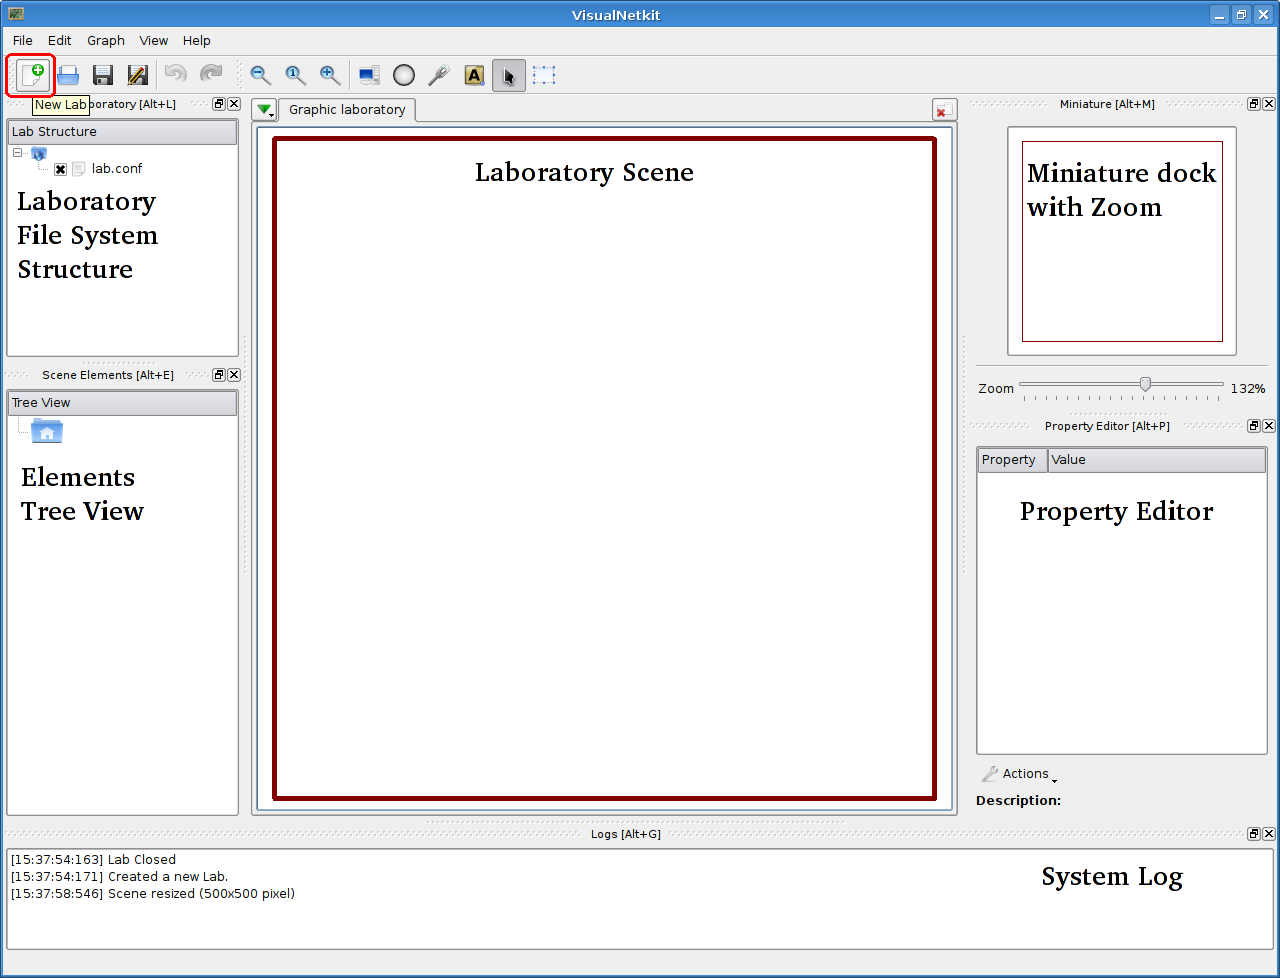
\includegraphics[width=12.5cm]{images/vnetkit_example1.png}
	\caption{Docks in \visualnetkit{}}
	\label{figura:vn_ex_dock}
\end{figure}

Le docks presenti - che comprendono anche le tool-bars -, sono tutte configurabili. L'utente può comodamente disporle a suo piacimento, nonché nascondere quelle che ritiene superflue.

Successivamente è possibile iniziare a costruire la topologia della rete in esame: utilizzando le apposite azioni presenti nel menu \emph{Graph}, l'utente può inserire nella scena grafica elementi quali Virtual Machines, Links, Collision Domain e Aree. Dapprima è necessario inserire le quattro \virtualmachine{} nella scena, attivando per l'host ``PC1'' anche il \plugin{} \emph{Test}, che verrà configurato in un secondo momento.

\begin{figure}[!htb]
	\centering
	\includegraphics[width=12cm]{images/vnetkit_example3.png}
	\caption{Inserimento dei links.}
	\label{figura:vn_ex_links}
\end{figure}

Al termine dell'operazione è possibile inserire il dominio di collisione posto a ``centro stella'', che andrà a collegare tutti gli host virtuali precedentemente creati. Infine, il lavoro sarà completato dall'inserimento dei links in cui verranno attivati i \plugin{} \emph{IPv4} e \emph{MAC}. Figura \ref{figura:vn_ex_links}.

Una volta realizzata la topologia di rete desiderata, il tool permette l'aggiunta di aree che possono essere utilizzate come etichette, oppure come aggregatori di elementi.

\subsection{Configurazione avanzata del laboratorio}
Spesso l'utente ha la necessità di configurare i servizi presenti all'interno degli host virtuali per garantire un corretto funzionamento delle macchine, al fine di effettuare con successo i test desiderati. \visualnetkit{} offre questa possibilità mediante l'uso della dock delle proprietà.
Quando si seleziona un elemento della scena grafica con un doppio click, il sistema provvede a renderizzare le informazioni dell'oggetto all'interno della property dock. Possiamo quindi trovare tutte le propietà presenti all'interno dei \plugin{} attivi per l'entità selezionata.

Alcuni moduli più complessi (nel caso dell'esempio il \plugin{} \emph{Test}) prevedono la possibilità di poter manipolare la struttura delle properties, in particolare questo avviene inserendo o eliminando sotto-attributi (figura \ref{figura:vn_ex_pp}).

\begin{figure}[!htb]
	\centering
	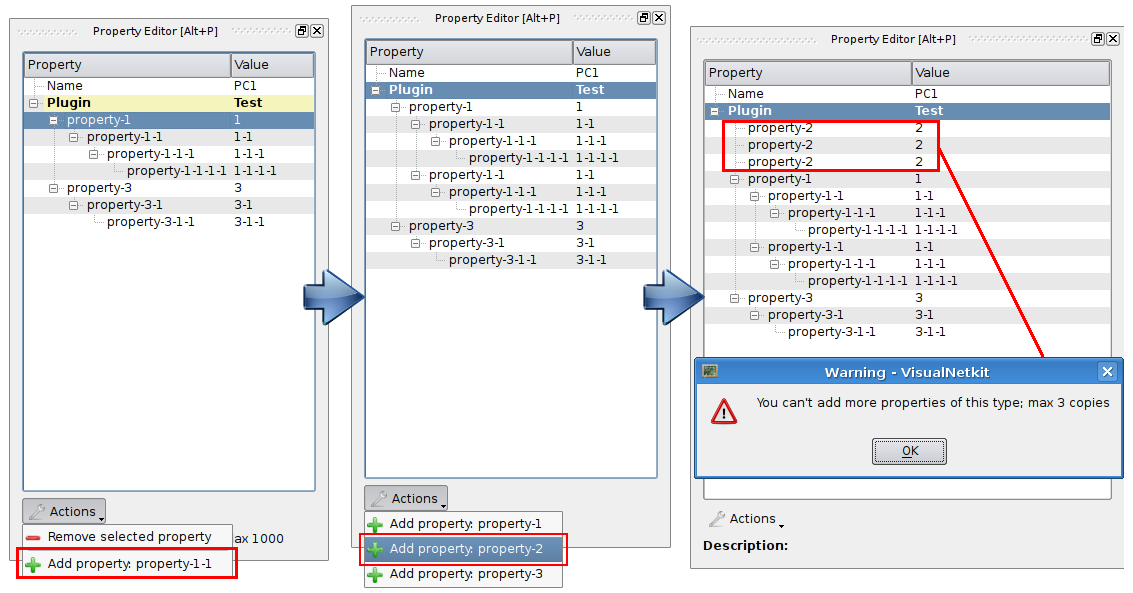
\includegraphics[width=13cm]{images/vnetkit_property_evolution.png}
	\caption{Modifica della struttura delle properties di un \plugin{}.}
	\label{figura:vn_ex_pp}
\end{figure}
Si vuole quindi modificare la struttura del modulo \emph{Test} attivo sulla macchina virtuale ``PC1''. Come mostrato, viene prima inserata una sotto-proprietà dell'attributo ``property-1'', successivamente si tenta di inserire tre copie della proprietà ``property-2'' che il modulo prevede.
Al tentativo di inserimento della quarta copia di quest'ultima, il \plugin{} restituisce un errore in quanto non sono previste più di tre duplicati per la proprietà in esame.

Tramite l'apposito bottone ``Actions'' è possibile, per ogni proprietà di un modulo, eliminare o aggiungere le sotto-property quando consentito. Quest'ultimo controllo, come quello inerente al controllo di cardinalità di una property poc'anzi citato, è interamente affidato al \plugin{}.

Il modulo analizzato nell'esempio è puramente utilizzato per il testing. Tuttavia, si può facilmente immaginare che un \plugin{} complesso, come \emph{Zebra} o \emph{Quagga}, possa avere una struttura simile a quella mostrata, il quale contiene molteplici attributi e sotto-attributi.

\subsection{Sperimentazioni sul laboratorio esportato}
Lo stadio finale della costruzione di un laboratorio mediante l'utilizzo di \visualnetkit{} si conclude con il salvataggio dello stesso sul \fs{}. Attraverso la voce \emph{Save As\ldots} presente nel menu \emph{File} è possibile selezionare la directory dove il Lab creato verrà esportato.

\begin{figure}[!htb]
	\centering
	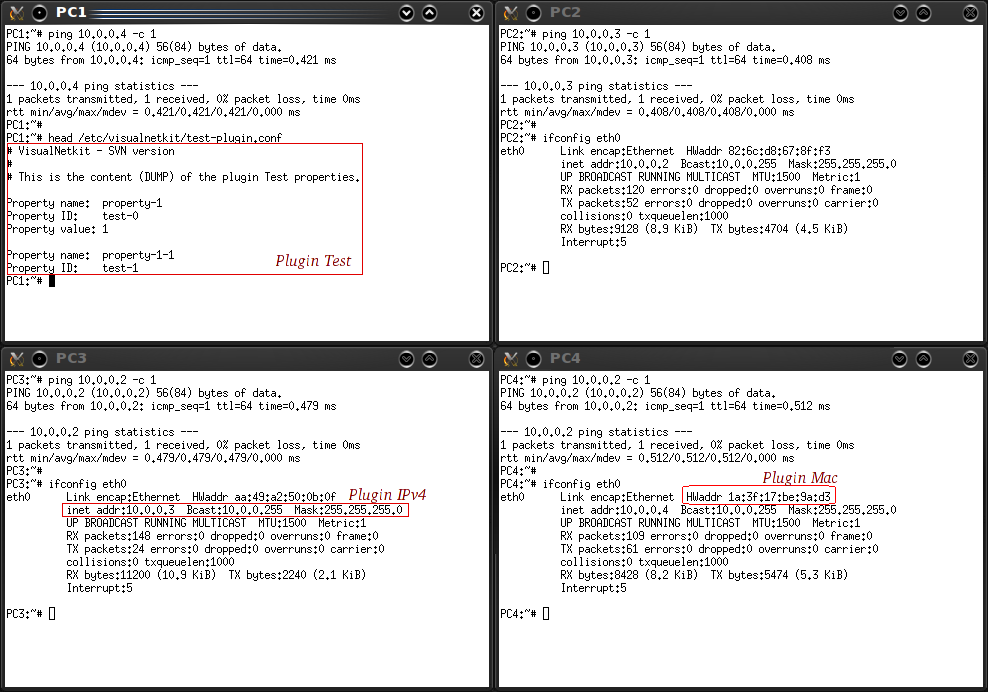
\includegraphics[width=13cm]{images/netkit_lab_example.png}
	\caption{Il laboratorio avviato emulato tramite \netkit{}.}
	\label{figura:ex_netkit}
\end{figure}

Effettuata questa operazione si può provvedere anche alla chiusura di \visualnetkit{}. Da questo momento in poi viene utilizzato \netkit{} per avviare la rete virtuale, in cui è possibile effettuare tutti i test che si desiderano.

Studiando il comportamento della rete precedentemente creata, è possibile osservare che il laboratorio esportato è completo in ogni dettaglio. Tutti gli host virtuali connessi ad un unico dominio di collisione riescono a colloquiare correttamente, come mostrato in figura \ref{figura:ex_netkit}. Inoltre, si può constatare che i \plugin{} attivati sui links e sull'host ``PC1'' hanno contribuito tutti a caratterizzare la parte della rete di propria competenza.

Ancora, è possibile immaginare un'estensione dell'architettura al fine di prevedere la possibilità di avviare un laboratorio direttamente da \visualnetkit{}, avendo la possibilità di mostrare all'utente una rappresentazione grafica dei terminali virtuali.

In ultima istanza, potrebbe risultare necessaria ed innovativa la realizzazione di un meccanismo che permetta ai vari moduli di comunicare e cooperare tra di loro; si pensi ad esempio, allo scenario in cui un modulo (attivo su una \virtualmachine) volesse conoscere tutti gli indirizzi IPv4 attivi sulle interfacce hardware presenti sull'host.
